\chapter{Introduction}

With the introduction of mathematical models, participation in financial markets evolved from an art to a science. Beginning with Harry Markowitz's modern portfolio theory, moving through the capital asset pricing model and the Black-Scholes option pricing model, modern finance is now replete with models for pricing derivatives, credit scores, and costs of capital; what was once speculation is now calculation. Crucially, models lead to algorithms, which remove human error and add the ability to digest large sets of data. 

The process of running computer algorithms to execute orders on an electronic exchange such as NASDAQ is known as \emph{algorithmic trading}. Speed of execution is typically crucial, often requiring running the algorithms on servers directly wired to the exchange, known as \emph{colocation}. Closely related is \emph{high-frequency trading}, which refers simply to the timescale, generally milliseconds, on which the algorithms submit orders. In theory, high-frequency trading is encompassed by algorithmic trading, while not all algorithmic trading need be high frequency; in practice, the two terms are often used interchangeably. 

The particular algorithms used in algorithmic trading vary greatly across the different types of strategies employed. Non-revenue-generating algorithmic trading is generally aimed at transaction cost reduction, with the primary theoretical papers on the subject being due to \citet{Bertsimas98} and \citet{Almgren01}. When an institutional investor wishes to buy or sell a large quantity of shares, the aim of the trader is to obtain the best possible price compared with some benchmark (often taken to be the midprice at the time of initiating the strategy). Here the term `large' is used relative to the liquidity of the stock - either in comparison to the average size of trades for the given stock, or to the available quantity to be bought/sold at the best listed price. The goal of the algorithmic trading strategy is then to split the large order into smaller pieces and execute them on an algorithmically determined schedule, balancing the total time for execution with the volatility of the price the trader will receive. 

Conversely, an example of algorithmic trading that capitalises on arbitrage opportunities to generate revenue is cross-exchange arbitrage, which uses simple, low-latency algorithms to profit from price discrepancies of a single stock dual-listed on two exchanges. The server running the algorithm is co-located at one of the exchanges, algorithm latency is on the order of microseconds, and the limiting reagent is the time taken for information to travel to and from the other exchange. In the case of Chicago and New York, for example, information can make the trip in 6 milliseconds via optical fibres that send information at about half the speed of light. For this reason, agents are now paying for access to a system of ground satellites that has been set up to relay information between the two exchanges via microwaves, shaving latency down to 4 milliseconds \citep{Laughlin14}. Another class of strategies for generating revenue using algorithmic trading are statistical arbitrage strategies, which use complex algorithms to profit from observed statistical patterns of a single stock on a single exchange. In statistical arbitrage, the aim is to exploit predictable statistical patterns in the available data provided by the exchange, such as predicting stock price movements from prices observed thus far. This method too requires colocation, and operates on the scale of milliseconds. It is this type of high-frequency trading that is explored in this dissertation. 

As part of the Dodd-Frank Act of 2010, the Volcker Rule has banned US banks from making certain speculative investments and, in so doing, effectively curbed their proprietary high frequency trading activity. Nevertheless, as they are still required to provide liquidity to markets via \emph{market-making} (simultaneously quoting both buy and sell prices on a range of financial instruments), banks use algorithmic trading to determine the bid/ask bands they will send to exchanges. Exploiting arbitrage opportunities using high frequency trading remains unrestricted for hedge funds, and notably has been used by Renaissance Technologies LLC's flagship Medallion fund to generate an average 71.8 percent annual return, before fees, from 1994 through mid-2014 \citep{rentech}. However, as it remains exclusive to only Renaissance employees and family members, it serves instead as a reminder of the revenue potential of high frequency algorithmic trading.

\section{The Limit-Order Book}

A \emph{limit order} is an instruction submitted by an agent to buy or sell up to a specified quantity or volume of a financial instrument, and at a specified price. A \emph{limit-order book (LOB)} is the accumulated list of such orders sent to a given exchange, where each order is accompanied by a timestamp and an anonymous key that uniquely identifies the agent. The exchange runs a trade-matching engine that uses the LOB to pair buy and sell requests that concur on price, even if only for partial volume. Orders remain in effect until they are modified, cancelled, or fully filled \citep{Kyle1989}.

The unfilled or partially filled orders accumulate in the limit-order book and provide liquidity to the market. At any given time, the structure of the LOB can be visualised as in \autoref{fig:LOB}. As new limit orders arrive, they are compared with existing opposing orders in the book in search of a match and, if so, existing orders are \emph{filled} (alternatively referred to as \emph{lifted}) according to a first-in-first-out priority queue for each price level. The price levels can also be referred to by their \emph{depth}, where the best bid and ask prices are called \emph{at-the-touch} and have a depth of zero, and depth increases in either direction according to the absolute price difference from the at-the-touch depths; the buy limit order at \$28.92 is at a depth of \$0.02. \emph{Market orders} extend the idea of limit orders by specifying only the volume, and accept the best possible price currently available in the LOB; whereas limit orders are free to post, modify, and cancel (as an incentive for providing liquidity), a fee is charged for executing a market order.

\begin{figure}
  \tikzsetnextfilename{Ch1/LOB}
  %\documentclass{article}
%\usepackage{pgfplots}
%\usetikzlibrary{backgrounds}
%\begin{document}
% Limit Order Book structure and mechanics by Anton, inspired by Ash Booth
\pgfdeclarepatternformonly[\LineSpace]{myhatch}{\pgfqpoint{-1pt}{-1pt}}{\pgfqpoint{\LineSpace}{\LineSpace}}{\pgfqpoint{\LineSpace}{\LineSpace}}%
{
    \pgfsetlinewidth{1pt}
    \pgfpathmoveto{\pgfqpoint{0pt}{\LineSpace}}
    \pgfpathlineto{\pgfqpoint{\LineSpace + 0.1pt}{-0.1pt}}
    \pgfusepath{stroke}
}

\newdimen\LineSpace
\tikzset{
    line space/.code={\LineSpace=#1},
    line space=5pt
}

\colorlet{buyLOcolor}{black!25}%
\colorlet{sellLOcolor}{black!90}%
\begin{center}%
\makebox[0pt]{%
\begin{tikzpicture}[
	/pgf/number format/fixed,
	/pgf/number format/fixed zerofill,	
	/pgf/number format/precision=2,
	buyLOone/.style ={rectangle,draw=black, fill=buyLOcolor,thick,outer sep = 0.05cm,minimum size=0.9cm,anchor=south,rounded corners=0.2cm},
	buyLOonematch/.style ={rectangle,draw=black,thick,outer sep=0.05cm,minimum size=0.9cm,anchor=south,rounded corners=0.2cm,preaction={fill=buyLOcolor},pattern=myhatch},
	buyLOtwo/.style ={rectangle,draw=black, fill=buyLOcolor,thick,outer sep = 0.05cm,minimum height =1.9cm ,minimum width=0.9cm,anchor=south,rounded corners=0.2cm},
	buyLOthree/.style ={rectangle,draw=black, fill=buyLOcolor,thick,outer sep = 0.05cm,minimum height=2.9cm,minimum width=0.9cm,anchor=south,rounded corners=0.2cm},
	sellLOone/.style ={rectangle,draw=black, fill=sellLOcolor,thick,outer sep = 0.05cm,minimum size=0.9cm,anchor=south,rounded corners=0.2cm},
	sellLOtwo/.style ={rectangle,draw=black, fill=sellLOcolor,thick,outer sep = 0.05cm,minimum height=1.9cm ,minimum width=0.9cm,anchor=south,rounded corners=0.2cm},
	sellLOthree/.style ={rectangle,draw=black, fill=sellLOcolor,thick,outer sep = 0.05cm,minimum height=2.9cm,minimum width=0.9cm,anchor=south,rounded corners=0.2cm}]
    \draw [>=latex,->] (-0.55,-0.05) -- (12,-0.05) node[draw=none,fill=none,midway,shift=(down:1),font=\Large] {Price};
    \draw [>=latex,->] (-0.55,-0.05) -- (-0.55,9) node[draw=none,fill=none,midway,rotate=90,shift=(up:0.75),font=\Large] {Volume};
    
    \foreach \x [evaluate=\x as \price using \x/100 + 28.90]  in {0,...,11} \draw (\x ,-0.05) -- (\x ,-0.1) node[anchor=north] {$\scriptstyle\pgfmathprintnumber{\price}$};

%%% LOB
	\node[buyLOone]			at (0,0) {};
	\node[buyLOone]			at (0,1) {};
	\node[buyLOtwo]			at (1,0) {};
	\node[buyLOone]			at (1,2) {};
	\node[buyLOthree]		at (2,0) {};
	\node[buyLOtwo]			at (3,0) {};
	\node[buyLOtwo]			at (3,2) {};
	\node[buyLOtwo]			at (3,4) {};
	\node[buyLOonematch]	at (4,0) {};
	\node[buyLOonematch]	at (4,1) {};
	\node[buyLOtwo] 		at (4,2) {};
	\node[buyLOone] 		at (4,4) {};
	
	\node[sellLOone]			at (7,0) {};
	\node[sellLOone]			at (7,1) {};
	\node[sellLOone]			at (7,2) {};
	\node[sellLOtwo]			at (8,0) {};
	\node[sellLOtwo]			at (10,0) {};
	\node[sellLOthree]		at (11,0) {};
	\node[sellLOthree]		at (11,3) {};

%%% BID ASK SPREAD
	\draw [<->] (5,1.5)  -- (6,1.5) node[midway, anchor=north, text width=2cm, align=center, thick] {Bid-Ask \\ Spread};

%%% MARKET ORDER		
	\node[sellLOtwo]			at (4,7) {};
	\draw[->, ultra thick] (4,7) -- (4,0.5);
	\node at (3.5,9) [anchor=north east, text width=3cm, align=right, font=\tiny] {A market order to sell two shares arrives, and matches with the first two limit orders in the queue at the best price.};
	
%%% LIMIT ORDER
	\node[sellLOone]			at (7,5) {};
	\draw[->, ultra thick] (7,5) -- (7,3);
	\node at (7.5,6) [anchor=north west, text width=2cm, align=left, font=\tiny] {A limit order to sell one share at 28.97 arrives, and is added to the back of the queue.};	
	
%%% LEGEND
	\node[buyLOone]			at (8,8) {};
	\node[sellLOone]			at (8,7) {};
	\node at (8.5,8.5) [anchor=west, align=left] {Bid (buy) LO};
	\node at (8.5,7.5) [anchor=west, align=left] {Ask (sell) LO};
\end{tikzpicture}
}
\end{center}
%\end{document}

%  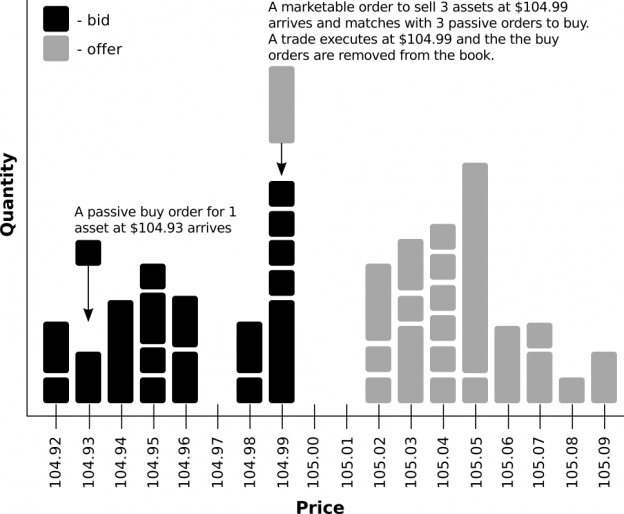
\includegraphics[width=0.9\textwidth]{Figs/LOBAshBooth.png}
\caption[Structure and mechanics of the limit-order book]{Structure and mechanics of the limit-order book, adapted from \citet{Booth15}. Each block represents an order, of varying volumes, submitted by various agents participating in the market.}
\label{fig:LOB}
\end{figure}

In the literature, LOBs are generally modelled in one of two ways: either by an economics-based approach or a physics-based approach \citep{Summary2013}. The economics-based approaches are trader-centric, assume perfect rationality, view order flow as static, and seek to understand trader strategies, in particular through game-style theories. By contrast, the physics-based approach, with which we are more concerned here, assumes zero-intelligence, provides simplified conceptual models of the evolution of the book, and is concerned with the search for statistical regularity. The dynamics of the book, namely order arrivals and cancellations, are governed by stochastic processes of varying complexity, from particles on a one-dimensional price lattice \citep{Bak97} to independent Poisson processes governing the arrival, modification, and cancellation of orders \citep{Cont10}. An excellent literature survey on LOB modelling can be found in \citet{Summary2013}.

\section{ITCH Data Set}
The underlying data that will be used in this work to generate imbalance and price change timeseries comes from the NASDAQ Historical TotalView-ITCH. ITCH\footnote{Remarkably, according to a representative of the NASDAQ, `ITCH' does not stand for anything.} is a  direct data-feed protocol that makes it possible for those with a paid subscription to track the status of every order from arrival until cancellation or execution. The Historical TotalView is simply a historical record of the events in the live feed. In the data used in this work, timestamps are provided to 1 millisecond, though newer versions of the feed offer nanosecond precision. Our data has been converted to MATLAB format; below, the structure of the event feed is described in detail (retaining only relevant fields):

\begin{table}[H]
\centering
\ra{1.2}
\begin{tabular}{@{} *{5}{c} @{}}
\toprule
Time & Order ID & Event & Volume & Price \\
\midrule
\vdots & \vdots & \vdots & \vdots & \vdots \\
39960699 &72408630 & 66 & 100 & 1107000 \\
39960710 & 72408630 & 68 & 100 & 1107000 \\
\vdots & \vdots & \vdots & \vdots & \vdots \\
\bottomrule
\end{tabular}
\label{tbl:ITCHevents}
\end{table}
{\bf Time:} Order arrival time in milliseconds from midnight. \\
{\bf Order ID:} Unique order reference number. \\
{\bf Event:} Event type:
\vspace{-\topsep}
\begin{itemize}[label={},nolistsep]
\item 66 -- Add buy order
\item 83 -- Add sell order
\item 69 -- Execute outstanding order in part
\item 67 -- Cancel outstanding order in part
\item 70 -- Execute outstanding order in full
\item 68 -- Delete outstanding order in full
\item 88 -- Bulk volume for the cross event
\item 84 -- Execute non-displayed order
\end{itemize}
\vspace{-\topsep}
{\bf Volume:} Number of shares. \\
{\bf Price:} Dollar price times 10,000. \par  
Thus, in the above example, we have a buy order arriving at 11:06am for 100 shares at \$100.70, and being cancelled 11 milliseconds later. From this feed we are able to reconstruct the entire limit-order book at any point in time, which amounts to being able to generate a plot as in \autoref{fig:LOB} detailing the exact liquidity available at each order depth.

\section{Order Imbalance}

A core component of this dissertation is limit-order book imbalance. \emph{Imbalance} is a ratio of limit order volumes between the bid and ask side, and in the work that follows is calculated as 
\begin{equation}\label{eq:LOBImbalance}
I(t) = \dfrac{V_{bid}(t) - V_{ask}(t)}{V_{bid}(t) + V_{ask}(t)}
\end{equation}
where $I(t) \in [-1,1]$, and both $V_{bid}$ and $V_{ask}$ are computed as the weighted average volumes at the three lowest depths having non-zero volume, using exponentially decreasing weights. As a sample calculation, the imbalance of the sample LOB presented in \autoref{fig:LOB} (prior to order arrivals) would be
\begin{align*}
V_{bid} & = \text{weight}(28.94)\cdot\text{volume}(28.94) \\
& \hphantom{{}={}} + \text{weight}(28.93)\cdot\text{volume}(28.93) \\
& \hphantom{{}={}} + \text{weight}(28.92)\cdot\text{volume}(28.92) \\
& = e^{-0.5 (0)} \cdot 5 + e^{-0.5 (1)} \cdot 6 + e^{-0.5 (2)} \cdot 3\\
& = 1.0000 \cdot 5 + 0.6065 \cdot 6 + 0.3679 \cdot 3 \\
& = 9.7428 \\
V_{ask} & = 4.9488 \\
I(t) & = \dfrac{9.7428 - 4.9488}{9.7428 + 4.9488} \\
&  = 0.3263
\end{align*}
In the figure we see that there are more limit orders on the bid side than on the ask, and the above value confirms that there is a medium imbalance in favour of the bid side.

\section{Roadmap}

Our objective in this dissertation is to use limit order book imbalance as a state variable in an algorithmic trading strategy, and to demonstrate that an effective statistical arbitrage strategy can be constructed around it. Our novel approach is to model imbalance and price change with a joint distribution, and to solve the resulting stochastic optimal control problem independently in both continuous time and discrete time.

The remainder of this dissertation is structured as follows:

{\bf Chapter 2} begins with the hypothesis that imbalance of bid/ask order volumes is an indicator for future price changes, and explores the possibility of constructing naive trading strategies using the statistical properties arising from modelling imbalance as a continuous time Markov chain; a basic understanding of probability theory is required. 

{\bf Chapter 3} casts the same statistical arbitrage problem into a stochastic optimal control framework, and solves it in both continuous and discrete time; familiarity with stochastic calculus and dynamic programming is assumed. 

{\bf Chapter 4} presents calibrations of the optimal controls and explores their dynamics. In-sample and out-of-sample backtests are conducted on historical ITCH data, which show a 877\% return on investment over 2014.

{\bf Chapter 5} concludes the dissertation by restating the primary backtesting results in the context of operational costs, and summarizes the key assumptions and simplifications that have been made. The conclusions are intended as considerations for future work on this topic.